\documentclass[../report.tex]{subfiles}


\begin{document}


\section{Introduction}
\label{introduction}

\subsection{Purpose}

This project focuses on the problem of creating a highly performant agent using Reinforcement learning techniques for the game Reversi. Reversi is a piece-capturing board game where disks are placed adjacent to existing opponent disks, capturing all consecutive opponent pieces between the new disk and the nearest ally disk. Similarily, the game Othello is a variation of this game, and has similar rules to Reversi and strategies within one usually carry over to the other.

Our implementation has a fixed starting state of 4 disks in the middle of the board in a square shape, where players take alternating turns. A player must place a disk such that it captures at minimum one opponent disk, skipping your turn if no legal move exists.

Due to the large variability of the game, with a large number of actions, states and possible ways to win, we decided that this game is a perfect candidate for various reinforcement learning strategies.
\begin{figure}[h]
    \caption{Two simple starting moves in Reversi.}
    \vspace{0.5cm}
    %\fbox{\rule[-.5cm]{0cm}{4cm} \rule[-.5cm]{10cm}{0cm}}
    \centering
    \begin{minipage}[t]{.30\textwidth}
        \centering
        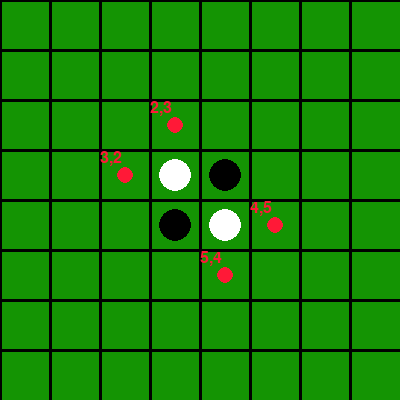
\includegraphics[width=\textwidth]{s1}
        \caption{Starting configuration in Reversi. Red dots signify the available moves the Black player is allowed to play}
    \end{minipage}
    \hspace{0.5cm}
    \begin{minipage}[t]{.30\textwidth}
        \centering
        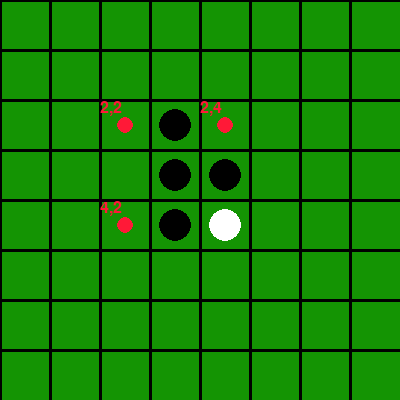
\includegraphics[width=\textwidth]{s2}
        \caption{Black player placed a disk at (2,3). Observe that a white disk was converted to a black disk}
    \end{minipage}
    \hspace{0.5cm}
    \begin{minipage}[t]{.30\textwidth}
        \centering
        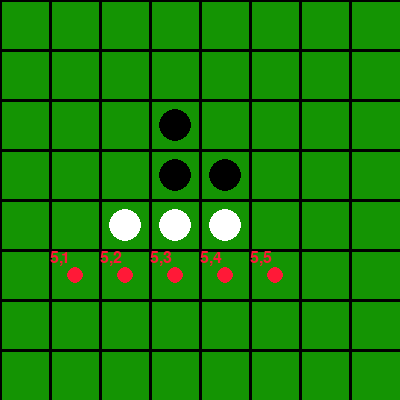
\includegraphics[width=\textwidth]{s3}
        \caption{White player placed a disk at (4,2). Observe that a black disk was converted to a white disk}
    \end{minipage}
\end{figure}

The game of Reversi ends when neither player can make a legal move, which typically means the game board is filled, but not always. Once the game has ended, the scoring is simple. The winner of Reversi is the player with the most game pieces on the board at the end of the game.


This problem is made complex by the $8\times8$ sized board which contains approximately $3^{64}$ possible states, each with a set of actions $\geq0$. With such a state and action space, tabular solutions are not practical, which makes different function approximation and Deep Reinforcement Learning solutions attractive. Since there are multiple methods to approach this problem, our project implements multiple algorithms and compares them against a baseline (Random) player and against each other. In particular, this project explores the effectiveness of Deep Q-Learning, and Deep SARSA. 

\subsection{Interests and Insights}

Since our problem is so similar to grid-based board games, our project may provide insights into the benefits and drawbacks of different Reinforcment Learning agents in this space.


Our project sources ideas for different function approximation algorithms from similar board games, and applied in insightful ways to  find the most optimal application of these algorithms. These insights can be then extended to other board games and possibly applied there as well.


In addition, the selection of multiple function approximation algorithms allows us to learn much more about the optimal learning methods, hyperparameters, and learning times for these different algorithms. Specifically, we can learn how algorithms taught with self-play interact with eachother or with the random agent and evaluate tailored learning methods for each algorithm.


In summary, there is a significant amount of knowledge in the development of this project that provides insights about Reinforcement Learning in Reversi. In addition, the insight gained in this project has the possibility of expanding beyond this specific problem into general problems in board and strategy games.


\subsection{Goal}
The goal of this report is firstly to detail to the reader the existing knowledge on Reversi in the Reinforcement learning space, then, we wish to impart multiple approaches to Reversi as a Reinforcement Learning problem, and to compare these approaches.

Finally, this report aims to use the empirical results gained through careful experimentation performed on the various methods to gain insights into the optimal algorithms and parameters of each approach.

\end{document}